% use the base acmart.cls
% use the sigplan proceeding template with the default 10 pt fonts
% nonacm option removes ACM related text in the submission. 
\documentclass[sigplan,nonacm]{acmart}
\usepackage{csvsimple}
\usepackage{subcaption}

\newcommand{\fixme}[1]{\textcolor{red}{#1}}
\newcommand{\todo}[1]{\textcolor{red}{TODO:\ #1}}
\newcommand{\fullname}{More Exact FPGA Technology Mapping with E-Graphs}
\newcommand{\shortname}{E-Pack}
\newcommand{\metric}{11\% fewer LUTs}
\newcommand{\fmetric}{46\%}
\newcommand{\B}{\mathbb{Z}_{2}}
\newcommand{\Bk}{\mathbb{Z}_{2}^{k}}
\newcommand{\Bx}[1]{\mathbb{Z}_{2}^{#1}}

% enable page numbers
\settopmatter{printfolios=true}


\begin{document}

\title{\fullname}

\begin{abstract}
    FPGA technology mapping is a well-studied problem and has been an area of
    interest in EDA tool design for decades. In most respects, the computational
    complexity of technology mapping is understood, and heuristic algorithms have
    been successfully employed to mitigate compile times while maintaining high QoR
    (quality of results). As transistor scaling comes to an end within the coming
    years, logic synthesis tools will become more of a bottleneck in the design of
    high performance accelerators. As a solution, we introduce E-Pack, an e-graph
    driven technology mapper that can better span the wide gap between SAT-based
    exact synthesis and heuristic cut enumeration techniques. We show that E-Pack
    can synthesize circuits with \metric{} on average---without ever
    increasing circuit depth. We also provide an empirical analysis of the runtime
    of E-Pack and show that it is still practical for large designs. Finally, we
    demonstrate that our compiler infrastructure is reusable, and future work can
    use our compiler for RTL equivalence checking or auditing the QoR of synthesis
    tools.
\end{abstract}
\maketitle % should come after the abstract

\section{Introduction}\label{sec:intro}
Given the complexity of modern electronic systems, a high degree of automation
is required to develop custom hardware within sensible timelines. At the
highest level, FPGA and ASIC design flows can be split into logic synthesis and
physical design (e.g., floorplanning placement and routing). This division of
work produces suboptimal designs, and neither are the individual synthesis
steps locally optimal on their own. However, circuit minimization problems in
general are NP-Hard~\cite{logicmin,twolevellogic}, and modern EDA flows bring
compile times down to the human timescale while maintaining acceptable quality
of results (QoR).

With the end of Dennard scaling and Moore's Law fading, the quality of logic
synthesis becomes more important. Hence, future synthesis tools will need to
expand the design spaces they explore and find more optimal solutions. Still,
finding provably optimal circuits is computationally intractable. In this
paper, we introduce how FPGA technology mapping can be augmented with e-graph
data structures to find \textit{more} exact solutions, without significantly
increasing compile times.

Technology mapping is the hand-off between logic synthesis and physical design.
It converts the abstract Boolean logic into a network of circuit elements that
belong to the target cell library. For FPGAs, the primary target cell is the
lookup table (LUT). Since every $k$-LUT can be re-programmed to satisfy any $k$
input boolean function, FPGA technology mapping has an unmistakably large
solution space. Whether the circuit is optimized for latency or area, most FPGA
tools approach technology mapping as a graph covering problem~\cite{flowmap,
    daomap, attmap, imap}. In the literature, a group of circuit nodes implemented
by a $k$-LUT is called a $k$-feasible cut of logic, and the generation of all
cuts is called cut enumeration. These structural mapping techniques rely on the
topology of the input circuit, and hence they are prone to \textit{structural
    bias}.

In contrast, functional mappers attempt to decompose the Boolean functionality
into smaller sub-functions which can be realized by $k$-LUTs. Such mappers are
a more exact approach, and often use SAT solvers to drive
synthesis~\cite{satmap,satmap2}. Other works employ Boolean matching to speedup
of technology mapping by identifying known Boolean
structures~\cite{boolmatch,fastboolmatch}. However, exact synthesis tools
cannot be scaled past tens of gates. As a consequence, cut enumeration and
functional mapping lie on two different extremes. The former is fast but
limited by the input structure, while the latter is unbiased but fundamentally
unscalable.

For this reason, we propose an e-graph driven technology mapper than can better
span the time-QoR spectrum. Equality graphs, referred to as e-graphs, are a
data structure which use union-find operations to compactly represent abstract
equivalence relations~\cite{eggpaper}. Whereas typical optimizing compilers
apply a greedy sequence of transformation passes, e-graphs rewrite terms
iteratively in a nondestructive fashion. Our work seeks to evaluate the
suitability of e-graphs for logic synthesis, specifically for technology
mapping to FPGAs. By using the output mappings of RTL synthesis tools as an
initial solution, we can use e-graphs to incrementally explore more compact
circuit topologies.

To that end, we propose \shortname{}: a tool for repacking FPGA netlists into
more compact forms---without increasing circuit depth. Our results show many
benchmarks, big and small, which synthesize to significantly fewer LUTs over
vendor EDA tools. To that end, our work makes the following contributions:

\begin{itemize}
    \item We formulate an intermediate language and set of e-graph rewrite rules that can
          explore circuit topologies that heuristic approaches miss.
    \item We evaluate our compiler against \nbenchmarks{} benchmarks combined from three
          sources: EPFL~\cite{epflbench}, ISCAS'85~\cite{iscasbench}, and
          LGSynth'91~\cite{lgsynthbench}. The results show improvements in LUT count
          without significant increases to compile time.
    \item Finally, \shortname{} is packaged as a Verilog-to-Verilog tool that can be
          dropped into existing RTL flows.
\end{itemize}

Before elaborating on our methodology and experimental setup, we first discuss
related ideas in technology mapping and e-graph driven compilers. Then, the
results section illustrates the typical reduction in LUT count our tool
achieves without increasing circuit depth. Lastly, we discuss the future work
of our compiler.
\section{Background and Related Work}\label{sec:relatedwork}
% Related work
% - e-syn
% - rover
% - egraphconstraints
% - dsd
% - adaptdecomp
\todo{explain related work}

\subsection{LUT Packing}\label{sec:relatedwork:packing}

\subsection{LUT Decomposition}\label{sec:relatedwork:decomp}

\subsection{E-Graph Superoptimization}\label{sec:relatedwork:egraph}
Equivalence graphs---e-graphs for short---are a data structure that were
originally conceived to facilitate automated proof generation. For example,
e-graphs can be used to simplify mathematical expressions~\cite{egraphmath} and
\todo{what cclemmadoes}~\cite{cclemma}. \todo{explain how EqSat works, why its
    good}. In recent years, e-graphs~\cite{eggpaper} and equality
saturation~\cite{eqsat} have enjoyed renewed popularity within the compilers
field. \todo{compiler examples}

\section{E-Graph Construction}\label{sec:rewrites}
The e-graph is built by accumulating new equivalence relations through the
iterative rewriting of terms. Rewrite rules define the equivalence relations in
full generality by designating a search pattern of terms to rewrite. The
right-hand side of the rule describes how to apply the rewrite to the pattern.
Rewrites must be merged back into the union-find data structure, so this is an
iterative process. Lastly, one needs to define a grammar that can represent the
structure of electronic circuits and lends itself well to pattern matching. As
an example, one can write De Morgan's laws as rewrite rule:

\begin{verbatim}
    (NOT (AND x y)) => (OR (NOT x) (NOT y))
\end{verbatim}

In the following subsections, we will define our netlist representation,
\texttt{LutLang}, and the accompanying equivalence relations. Formalizing the
meaning of FPGA netlists is critical to both ensuring correctness and finding
deeper insight into the structure of our rewrite rules under composition.

\subsection{\texttt{LutLang} Representation}\label{sec:rewrites:lutlang}

Our compiler has a custom Verilog frontend for the sake of converting netlists
to a format, called \texttt{LutLang}, that is compatible with e-graph
structures. When printed to text, \texttt{LutLang} takes on a Lisp-like syntax
and our rewrite rules are written in such style. As an example, a 2-LUT
cascaded into a 3-LUT is written as follows:

\begin{verbatim}
    (LUT F x2 x3 (LUT G x0 x1))
\end{verbatim}

\texttt{F} and \texttt{G} are the truth-tables of the LUTs.
We also call them the \textit{program} or \textit{function} interchangeably.
Since $k \leq 6$, truth tables are stored with 64-bit integers, but we analyze them as total functions from $\Bk \rightarrow \B$.
To clarify notation, $\mathbb{Z}_2 = \mathbb{Z}/2\mathbb{Z} = \mathbb{B} = \{0,1\}$.
To that end, the semantics of a LUT is simply applying its boolean inputs to the function:

\begin{equation}
    \llbracket \texttt{(LUT G x0 x1)} \rrbracket = G(\llbracket \texttt{x0} \rrbracket, \llbracket \texttt{x1} \rrbracket)
\end{equation}

\begin{figure}
    \centering
    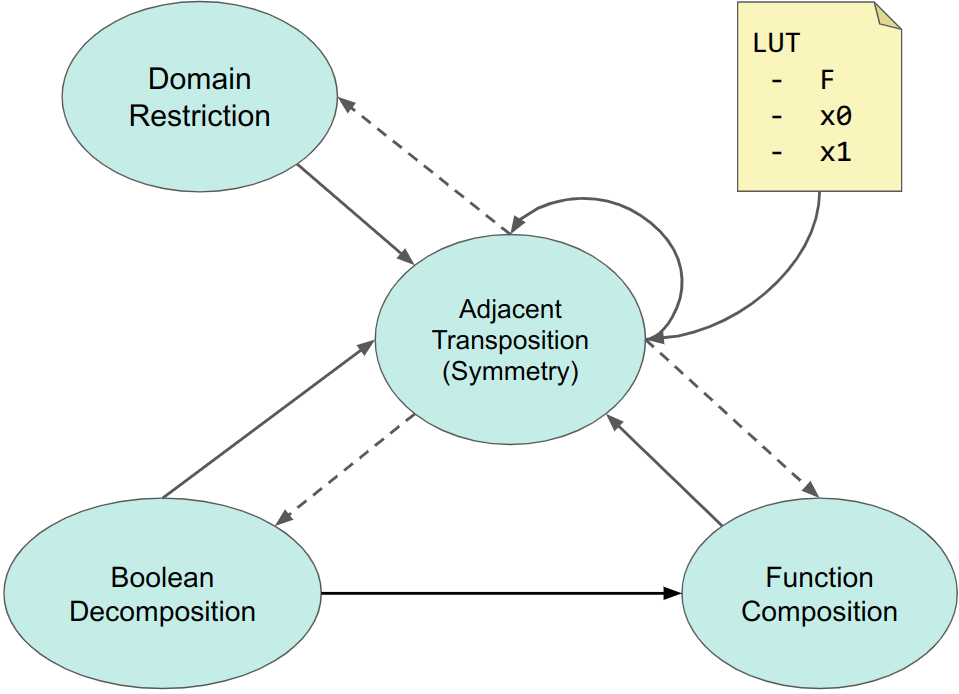
\includegraphics[width=0.47\textwidth]{img/rewrites.png}
    \caption{Transition diagram of rewrite rules. A solid arrow means that the application of the source rule always becomes an instance of the target rule.}\label{fig:rewrites}
    \Description[]{}
\end{figure}

\subsection{Simplifying Degenerate LUTs}\label{sec:rewrites:degen}

\textbf{Definition:} A LUT's configuration $F : \Bk \rightarrow \B$ is \textit{degenerate} if there exists a Shannon expansion $F = x_i \cdot F_{x_i} + \overline{x_i} \cdot F_{\overline{x}_i}$
such that $F_{x_i} = F_{\overline{x}_i}$ for some $i \in \{ 0, \ldots, k -1\}$. In other words, $F = F_{x_i} = F_{\overline{x}_i}$.

The output of a degenerate LUT is not dependent on one of its inputs. Hence, it
can be rewritten into a LUT which uses fewer inputs. This rule is applied by
computing the Shannon expansions of LUTs and checking for equivalence. For
$k=3$, the rules takes on the following form:

\begin{verbatim}
    (LUT F x0 x1 x2) => (LUT F' x0 x1)
        if F(x0, x1, false) == F(x0, x1, true)
        where F'(x0, x1) := F(x0, x1, true)
\end{verbatim}

To the left of \texttt{=>} is the \textit{search pattern}. The right-hand side
of the rule is the \textit{application}. One rule is instantiated for each LUT
size $k =1$ through 6. One should notice that LUTs which are constant functions
are also handled by this rule. Since this rule is computationally expensive, it
is applied greedily as a pre-processing step before the e-graph is built. None
of the other rewrite rules create degenerate LUTs, so this has no impact on
results. Of course this rule can be enabled at any time, if it were necessary.

\subsection{Partial Application}\label{sec:rewrites:application}
A LUT with a constant input can be partially evaluated to a LUT with one less
input. This rule is similar to the last. It computes the Shannon expansion
along the constant variable and chooses the cofactor that matches the state of
the constant input. Applying this rule greedily in combination with the
previous one is equivalent to constant propagation. As an example, the
pseudocode for $k=3$ is written as follows:

\begin{verbatim}
    (LUT F x0 x1 false) => (LUT F' x0 x1)
        where F'(x0, x1) := F(x0, x1, false)
\end{verbatim}

\subsection{Functional Composition}\label{sec:rewrites:composition}

Cascaded LUTs can be packed into a single LUT, as long as the size of the cut
of logic has at most 6 leaf nodes. For instance, a circuit that implements
$F(x_0, x_1, G(x_2, x_3))$ with a 3-LUT and 2-LUT can be rewritten as a 4-LUT
that implements some $H(x_0, x_1, x_2, x_3)$. In pseudocode, this would take on
the following form:
\begin{verbatim}
    (LUT F x0 x1 (LUT G x2 x3)) => (LUT H x0 x1 x2 x3)
        where H(x0, x1, x2, x3) := F(x0, x1, G(x2, x3))
\end{verbatim}

The search patterns \texttt{x0} and \texttt{x1} can match any node. They are
not necessarily principal inputs, and hence can be outputs from other LUTs. As
a consequence, this rule can be chained together many times in varying orders
to pack a sub-circuit into a single LUT. As demonstrated in the next section,
we can write this rule for one specific input position, without loss of
generality. Therefore, we only need to sweep over the size of the two LUTs in
the search pattern. In total, there are $6*6 = 36$ LUT packing rules. When the
cut of logic is larger than 6 leaves, the rules fail gracefully and do not
interfere with reaching equality saturation.
\subsection{LUT Symmetries}\label{sec:rewrites:symmetry}

The semantics of LUTs should not depend on the order of their inputs. If two
LUTs have permuted inputs but are otherwise functionally identical, they should
belong to the same e-class in the graph. That is, \mbox{\texttt{(LUT F .. xi ..
        xj ..)}} is semantically equivalent to \mbox{\texttt{(LUT G .. xj .. xi ..)}}
if and only if $G = F \odot \sigma^{-1}$, where $\sigma \in S_k$ is the
permutation applied to the inputs.

\begin{proof}
    $\odot$ is a right-action defined for the sake of permuting the inputs to a function before they are applied:
    \begin{equation*} \odot : \big (\Bk \rightarrow \mathbb{Z}_2 \big ) \times S_k \rightarrow \big (\Bk \rightarrow \mathbb{Z}_2 \big ) \end{equation*}
    \begin{equation*} F \odot \sigma : (x_0, x_1, \ldots, x_{k-1}) \mapsto F(x_{\sigma(0)}, x_{\sigma(1)}, \ldots, x_{\sigma(k-1)}) \end{equation*}

    It is trivial to prove that this right-action is associative:
    \begin{align*}
        (F \odot \sigma_1) \odot \sigma_2 & = F(x_{\sigma_2(\sigma_1(0))}, x_{\sigma_2(\sigma_1(1))}, \ldots, x_{\sigma_2(\sigma_1(k-1))}) \\
        (F \odot \sigma_1) \odot \sigma_2 & = F \odot (\sigma_2 \circ \sigma_1)
    \end{align*}
    With this property, the rest follows directly:
    \begin{equation}
        F = G \odot
        \sigma \iff F \odot \sigma^{-1} = (G \odot \sigma) \odot \sigma^{-1} = G
    \end{equation}
\end{proof}

Therefore, we can conclude that $k$-LUTs have as much symmetry as can be
generated by the group $S_k$. This formal approach may be considered overkill,
but it has two major consequences. First, it precisely reveals how many e-graph
rewrite rules are needed to generate all the symmetries of a LUT. For any
$k$-LUT with program $F$, we need exactly as many rules as it takes to generate
$F \odot S_k$. It is a well-known fact in algebra that the $k-1$ adjacent
transpositions generate $S_k$~\cite{sgroup}. Therefore, we can insert an
e-graph rewrite rule for each adjacent transposition. In total, this is
$\sum_{k=2}^{6} (k-1) = 15$ rules to encapsulate symmetry for every LUT size.
The second consequence is that every other rewrite rule can now be defined for
one input position, without loss of generality. This reduces the total number
of rewrite rules, making it easier to rationalize about the rule system and
which types of optimizations are reachable.

\subsection{LUTs with Domain Restrictions}\label{sec:rewrites:restrict}

\textbf{Definition:} A lookup table \texttt{(LUT F x0 x1 \ldots)} is \textit{restricted} if \texttt{xi == xj} for some $ i, j \in \{0, \ldots, k-1\}, \; i \neq j$.
In other words, the domain of the LUT is restricted.

The main advantage of using e-graphs is the compact way in which it represents
notions of equality. When considering the entire set of rewrite rules under
composition, we can observe new equalities being formed in the e-graph.
Whenever an equality is found between two of the inputs to a $k$-LUT, it can be
rewritten with a $(k-1)$-LUT. We simply need to define and compute
$\texttt{restrict(F, i, j)}$ which maps $F : \Bx{k} \rightarrow \B$ to the
domain-restricted $F \vert_{x_i = x_j} : \Bx{k-1} \rightarrow \B$. In
pseudocode, the rewrite rule can be rewritten as follows:

\begin{verbatim}
    (LUT F x0 x1 x1) => (LUT G x0 x1)
        where G := restrict(F, 1, 2)
\end{verbatim}

Since e-graph rewrite patterns search on e-classes, this rule is automatically
re-checked when e-classes are merged. Since LUT symmetry is represented in the
graph, only one rule is needed for each lut size $k=2$ through 6.

\subsection{Functional Decomposition}\label{sec:rewrites:decomp}

Decomposing boolean functions and logic minimization in general is
NP-complete~\cite{logicmin}. Correspondingly, decomposing LUTs explodes the
size and build time of the e-graph. However, we can still define rewrites that
look for fully disjoint decompositions in one or more variables. This rule has
no structural element to search for, so it runs every time an e-class is
updated. Our implementation computes the Shannon expansion of a $k$-LUT's
function $F$ and checks that both cofactors are cognates in a loose sense. For
instance, given $k=3$ then it is true that:

\begin{gather}
    F(x_0, x_1, x_2) = G(x_0, H(x_1, x_2)) \nonumber \\
    \Big\Updownarrow                       \nonumber \\
    F_{x_0} (x_1, x_2) = G_{x_0} (H(x_1, x_2)) \land F_{\overline{x}_0} (x_1, x_2) = G_{\overline{x}_0} (H(x_1, x_2))
\end{gather}

In practice, our implementation checks if either of the cofactors are constant
functions or if the cofactors are equivalent up to complementation.

\subsection{Register Retiming}\label{sec:rewrites:retiming}

\begin{figure*}[tb]
    \begin{subfigure}{0.33\textwidth}
        \centering
        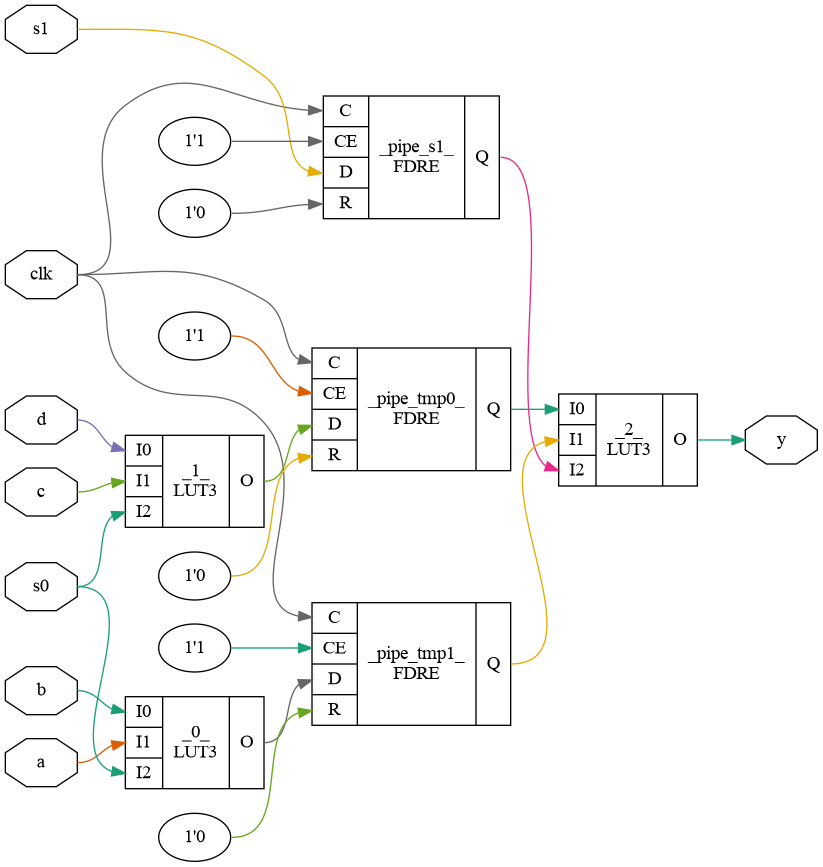
\includegraphics[width=\textwidth]{img/mux_4_1.png}
        \caption{Three 3-LUT, three FF topology.}\label{fig:retiming:a}
        \Description[]{}
    \end{subfigure}
    \begin{subfigure}{0.33\textwidth}
        \centering
        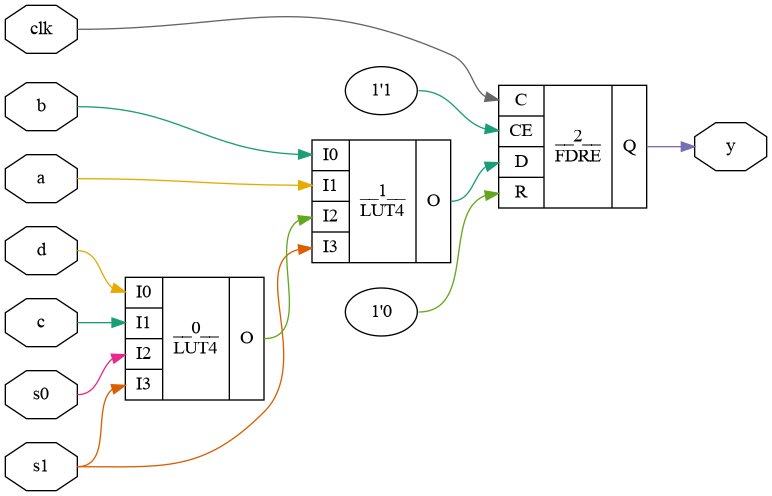
\includegraphics[width=\textwidth]{img/mux_4_1_retime_dsd.png}
        \caption{Two 4-LUT, one FF topology.}\label{fig:retiming:b}
        \Description[]{}
    \end{subfigure}
    \begin{subfigure}{0.33\textwidth}
        \centering
        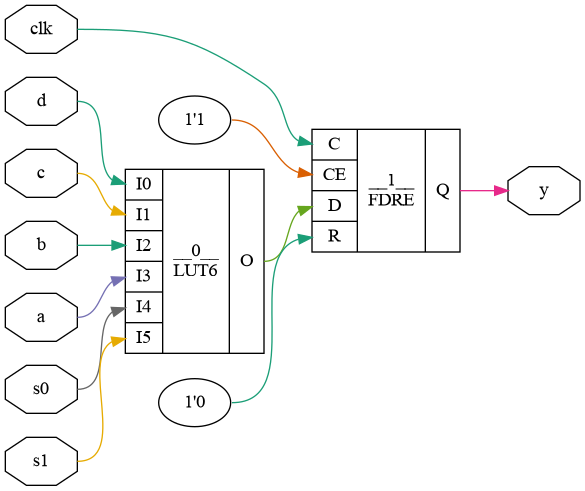
\includegraphics[width=\textwidth]{img/mux_4_1_retime.png}
        \caption{One 6-LUT, one FF topology.}\label{fig:retiming:c}
        \Description[]{}
    \end{subfigure}
    \caption{Three varying topologies for 4:1 MUX with pipeline register. \todo{Placeholder images. Remake by hand.}}\label{fig:retiming}
    \Description[]{}
\end{figure*}

Register retiming, as a purely structural rule, can be implemented with a
simple search and apply pattern. An example for $k=3$ would be written as
follows:

\begin{verbatim}
    (LUT F (REG x0) (REG x1)) <=> (REG (LUT F x0 x1))
\end{verbatim}

Unlike the other rules, this rule is searched for in both directions.
Figure~\ref{fig:retiming} illustrates an example of how register retiming can
compose with LUT rewrite rules to reduce LUT count and register count
simultaneously. In this case, LUTs representing 2:1 multiplexers are push
across register boundaries. Since this logic happens to have a one 6-LUT
packing and two 4-LUT packing, the total LUT count is reduced in conjunction
with register count. Moreover, our cost model can take into account different
weights for flip-flop cells versus LUT cells. E-graph extraction is elaborated
in the next section, but it should be noted that our trials weight LUTs and
registers equally.
\section{Tool Flow}\label{sec:flow}

While constructing the e-graph is the crux of \shortname{}, there are several
other important components to consider in the full design flow. In order to
test our hypothesis, \shortname{} must be compatible with existing synthesis
flows, and attempts at finding reduced circuits must be verified.

\begin{figure}
    \begin{subfigure}{0.47\textwidth}
        \centering
        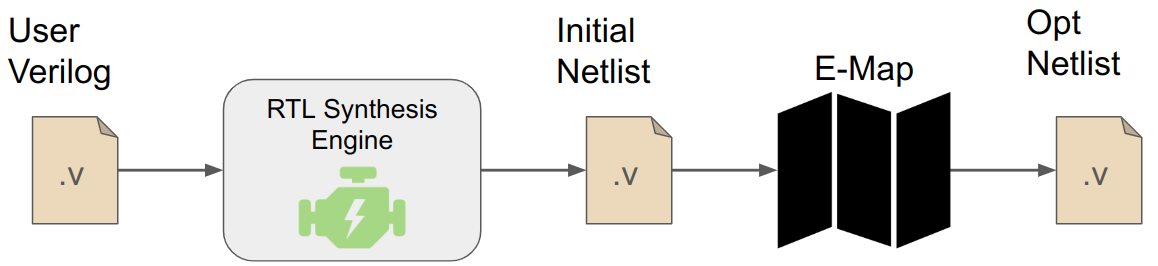
\includegraphics[width=\textwidth]{img/flow.png}
        \caption{Tool flow to integrate E-Pack with existing RTL synthesis engines. \todo{figure text is incorrect}}\label{fig:flow:rtl}
        \Description[]{}
    \end{subfigure}
    \hfill\vspace{4mm}
    \begin{subfigure}{0.47\textwidth}
        \centering
        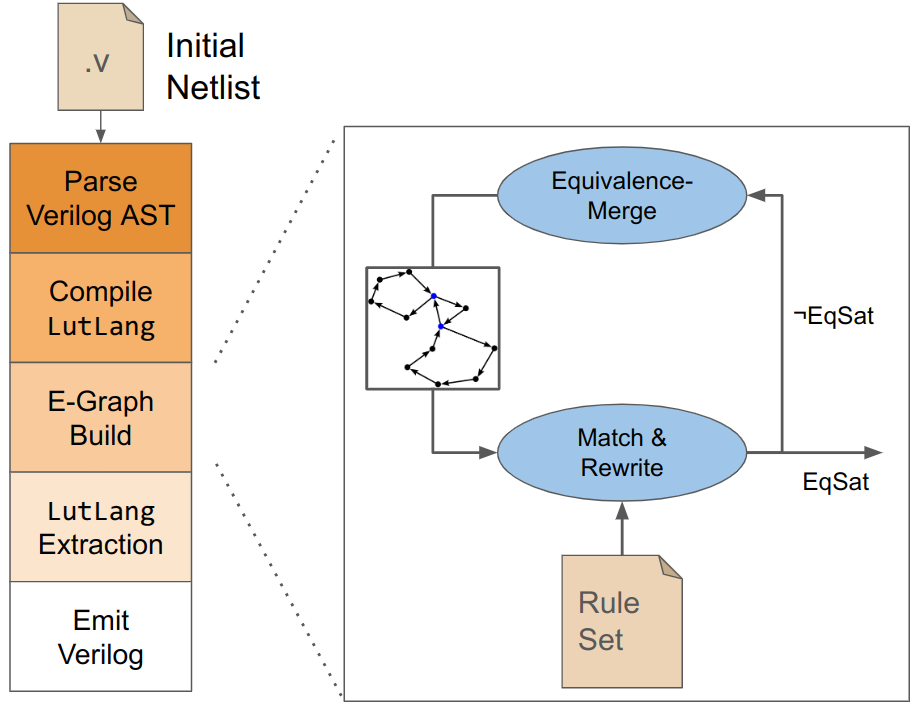
\includegraphics[width=\textwidth]{img/egraph.png}
        \caption{Compilation steps internal to \shortname{} Verilog tool.}\label{fig:flow:egraph}
        \Description[]{}
    \end{subfigure}
    \caption{\todo{root caption}}\label{fig:flow}
\end{figure}

\subsection{Extraction}\label{sec:flow:extraction}
Regardless of whether equality saturation is achieved or not, the quality of
the output circuit still largely depends on the extraction technique used. In
short, \textit{extraction} is the process of selecting the ``best'' circuit
from the e-graph. Given that a saturated e-graph can contain hundreds of
thousands of e-nodes across tens of thousands of e-classes, a greedy extraction
algorithm is the most pragmatic. The greedy extractor iterates over the
e-classes, updating the cost of the cheapest e-node until the database of costs
no longer change. Whenever possible, our compiler uses the builtin
functionality of the egg e-graph Rust library~\cite{docsEgg}. However, e-graph
extraction itself is an ongoing research area~\cite{smoothe,
    sparsextract,esynth}, and future work would experiment with different
extraction algorithms. In any case, the cost of a LUT is always one plus the
sum of the costs of its children nodes. The subtle interactions between
extraction and the rewrite rule set are further explained in
Section~\todo{result sec}.

\subsection{Verilog Support}\label{sec:flow:verilog}
In order for our compiler to be compatible with as many existing design flows
as possible, some level of Verilog support is necessary. Our compiler supports
an ad-hoc subset of Verilog 2001~\cite{verilog}, as required to represent
structural netlists. This includes support for non-ANSI C style module
delcarations, wires, and module instantiations with named port connections.
With Verilog support, we are able to test \shortname{} with tool flows that use
Yosys~\cite{yosys} or Vivado~\cite{vivado}. On the backend, our compiler also
emits an updated Verilog netlist.

\subsection{Verification}\label{sec:flow:verification}
While verification is the not the primary focus of this work, some level of
validation is required to build trust in our synthesis results. In fact,
e-graphs were originally designed for automated theorem
proving~\cite{eggpaper}. Thus, constructing proofs that demonstrate equivalence
between the original and optimized netlist is a builtin feature of
\shortname{}. However, this technique is relatively slow, so we use two other
independent sources of verification. For combinational netlists, our middle end
can do exhaustive functional testing. Lastly, we use Yosys~\cite{yosys} for its
SAT-driven equivalence checking capabilities. All in all, the mixed usage of
these verification techniques build great confidence in the robustness of our
technology mapper built around e-graphs.
\section{Results}\label{sec:results}
For our experiments, we used a Red Hat 8 server with a Intel Xeon Gold 6242
CPU. Since \shortname{} is written in Rust, it mostly uses the built-in
functionality of the egg library. The egg e-graph runner was ran in a
time-limited configuration, meaning there was no limit in the size of the
e-graph or number of rewrite iterations. The specific time limit for e-graph
construction was 10 minutes. In most cases, the test circuit saturated the
e-graph before this time limit. \shortname{} was evaluated against circuits
from three benchmark suites: EPFL~\cite{epflbench}, ISCAS'85~\cite{iscasbench},
and LGSynth'91~\cite{lgsynthbench}. However, we also included an ALU and
pipelined multiplication module to test how our compiler behaves with
increasing levels of bit-parallelism and pipeline stages. Finally, we measure
how our mapping optimizations influence timing closure.

\subsection{Benchmarking}\label{sec:results:benchmark}
\begin{table}
    \centering
    \csvautobooktabular{data/results.csv}
    \caption{Results of 30 improved benchmarks from ISCAS'85, LGSynth'91, and EPFL}\label{tab:results}
\end{table}
Among the 96 benchmarks we tested, we found that \shortname{} was able to
reduce the LUT count \fmetric{} of the time. On average, \shortname{} packed the
netlists to \metric{}. The results in Table~\ref{tab:results} list the LUT counts \todo{explain table}.

\subsection{Marginal Improvement and Time Cost}\label{sec:results:margin}
\begin{figure}
    \begin{subfigure}{0.47\textwidth}
        \centering
        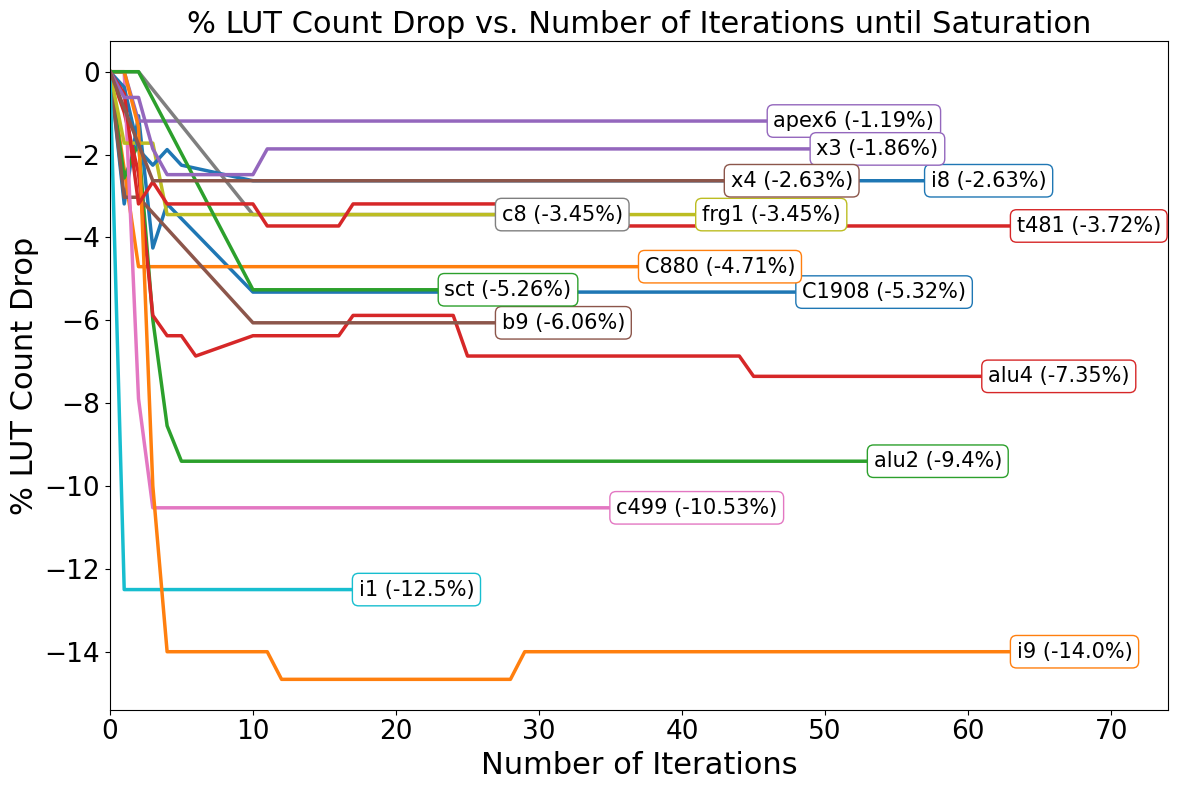
\includegraphics[width=\textwidth]{img/improvement.png}
        \caption{Marginal improvement versus iteration count. The labels mark the equality saturation point.}\label{fig:marginal:improvement}
        \Description[]{}
    \end{subfigure}
    \hfill\vspace{4mm}
    \begin{subfigure}{0.47\textwidth}
        \centering
        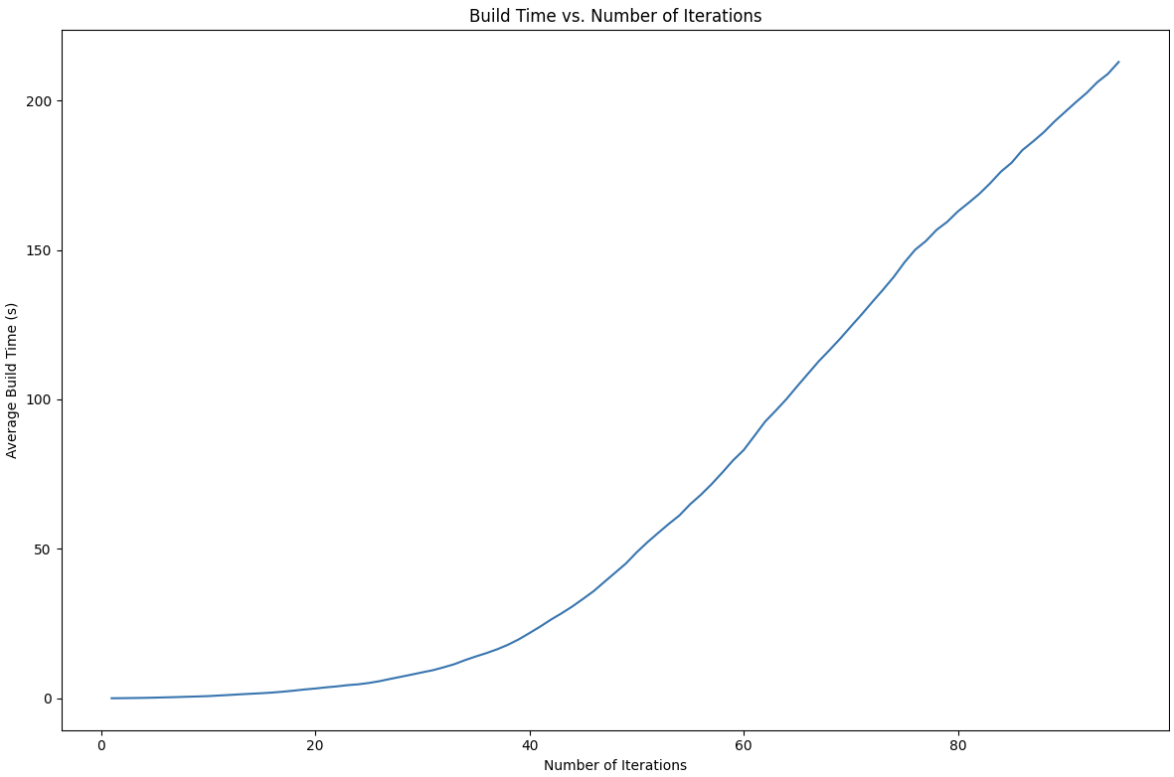
\includegraphics[width=\textwidth]{img/runtime.png}
        \caption{Marginal increase in runtime versus iteration count. Longer iterations consume more time as the graph is larger.}\label{fig:marginal:runtime}
        \Description[]{}
    \end{subfigure}
    \caption{Comparison between gains in QoR against increasing execution time with graph size. Running a netlist to equality saturation requires more rewrite iterations, and hence a larger e-graph.}\label{fig:marginal}
    \Description[]{}
\end{figure}
\todo{explain graph showing improvement with iter count}

\subsection{Case Study: Pipelined Designs}\label{sec:results:retiming}
\begin{table*}[t]
    \centering
    \csvautobooktabular{data/mult.csv}
    \caption{\todo{mult captiofn}}\label{tab:multiply}
\end{table*}
\todo{explain pipelined mult design}

\subsection{Case Study: Bit-Parallel Designs}\label{sec:results:scalability}
\begin{table}
    \centering
    \csvautobooktabular{data/alu.csv}
    \caption{Synthesis results of $n$-bit ALU}\label{tab:alu}
\end{table}
\todo{explain increasing ALU bit parallelism}

\section{Conclusion and Future Work}\label{sec:conclusion}
\todo{write the conclusion}

% Unstarted sections:
% [ ] Mult results: a big opportunity, but greedy extraction somewhat ruins it
% [ ] Future work

% Unstarted figures:
% [ ] A rewritten circuit (re-make by hand)

% MISC TODOS:
% (Matt): Explain the bumps and dips in the plot
% (Matt): Explain somewhere (prob results) that iterations/time *sometimes* mattter
% (Matt): Explain/mention rewrite figure in text

% use the ACM bibliography style
\bibliographystyle{ACM-Reference-Format}
\bibliography{references}

% \newpage
%%
%% If your work has an appendix, this is the place to put it.
% \appendix

\end{document}